\chapter{Implementation} % The implementation should look at any issues you encountered as you tried to implement your design. During the work, you might have found that elements of your design were unnecessary or overly complex; perhaps third party libraries were available that simplified some of the functions that you intended to implement. If things were easier in some areas, then how did you adapt your project to take account of your findings? It is more likely that things were more complex than you first thought. In particular, were there any problems or difficulties that you found during implementation that you had to address? Did such problems simply delay you or were they more significant? You can conclude this section by reviewing the end of the implementation stage against the planned requirements.

@TODO - style guide


\section{SmartResolution directory structure}

As the implementation followed an agile methodology, the design evolved over time and thus, the directory structure could not be determined up-front. Most (but not all) of the key directories and folders are outlined below:

\begin{samepage}
\dirtree{%
.1 data/.
.1 features/.
.1 test/.
.1 vendor/.
.1 webapp/.
.2 core/.
.3 api/.
.3 controller/.
.3 db/.
.3 model/.
.3 view/.
.2 modules/.
.3 other/.
.3 config.json.
.2 uploads/.
.2 index.php.
.2 routes.php.
.1 .travis.yml.
.1 composer.json.
.1 Gemfile.
}
\end{samepage}

\lstinline{data} contains fixture data for tests. This is also where the test and production SQLite3 databases reside.

\lstinline{features} contains the Cucumber features and Ruby step definitions.

\lstinline{test} contains all PHP unit tests.

\lstinline{vendor} is an automatically generated directory, created by Composer, containing all of SmartResolution's dependencies.

\lstinline{webapp/core} contains the core ODR platform, which uses an MVCR compound design pattern (\lstinline{webapp/routes.php} defines the routing component). The \lstinline{model}, \lstinline{view} and \lstinline{controller} directories are self-explanatory.

Also inside the core is the \lstinline{db} directory, which contains middleware classes connecting the model classes to the database, since models should encapsulate the concept of whatever it is they are representing, rather than being responsible for the relational database to object mapping.

Finally, this folder also contains an \lstinline{api} directory, which defines all of the global functions available to modules. Having these in their own directory made generating module-specific API documentation easy.

Going back up a level, we have \lstinline{webapp/modules}, which contains any installed SmartResolution modules. This is where the maritime collision module resides once it has been installed. A \lstinline{config.json} file (edited in a user-friendly way through the admin dashboard) denotes which modules are installed and whether or not they are active.

Finally, at the top level we have a few interesting files:

\lstinline{.travis.yml} - an instructions file for Travis Continuous Integration, describing how to set up the project and run its tests.

\lstinline{composer.json} - describes SmartResolution's dependencies. Developers can install all dependencies simply by running \lstinline{composer install}.

\lstinline{Gemfile} - describes SmartResolution's Ruby dependencies. Required for the Cucumber and Ruby integration tests.

\section{Class diagrams}

The system was developed in an agile way, hence these class diagrams are not in the design section but the implementation section. What evolved from the design was a state pattern representing the current state of a dispute.

\subsection{State pattern}

Please refer to figures~\ref{uml:activity:dispute} and~\ref{uml:activity:mediation} for a reminder of the workflow of a dispute. These diagrams alluded to the fact that disputes can be in different states. This was something that was eventually carried over to the implementation of the code.

In early versions of the project, the codebase began to get quite messy because various classes throughout the system were dependant on the state of a dispute to decide whether or not they could perform an action. This led to complicated if statements, like the one below:

\begin{lstlisting}
if ($dispute->state() === 'Open' || $dispute->state() === 'InMediation' || $dispute->state() === 'NegotiatingLifespan') {
    doSomething();
}
\end{lstlisting}

Figure~\ref{uml:states} shows how the state pattern was adopted to overcome problems like this. Classes throughout SmartResolution could now query the dispute's state directly, as the responsibility of whether or not an action could be performed was encapsulated inside the state itself. The above example could thus be rewritten as follows:

\begin{lstlisting}
if ($dispute->state()->canDoSomething()) {
    doSomething();
}
\end{lstlisting}

\begin{figure}[h!]
  \centering
    \ifimages
    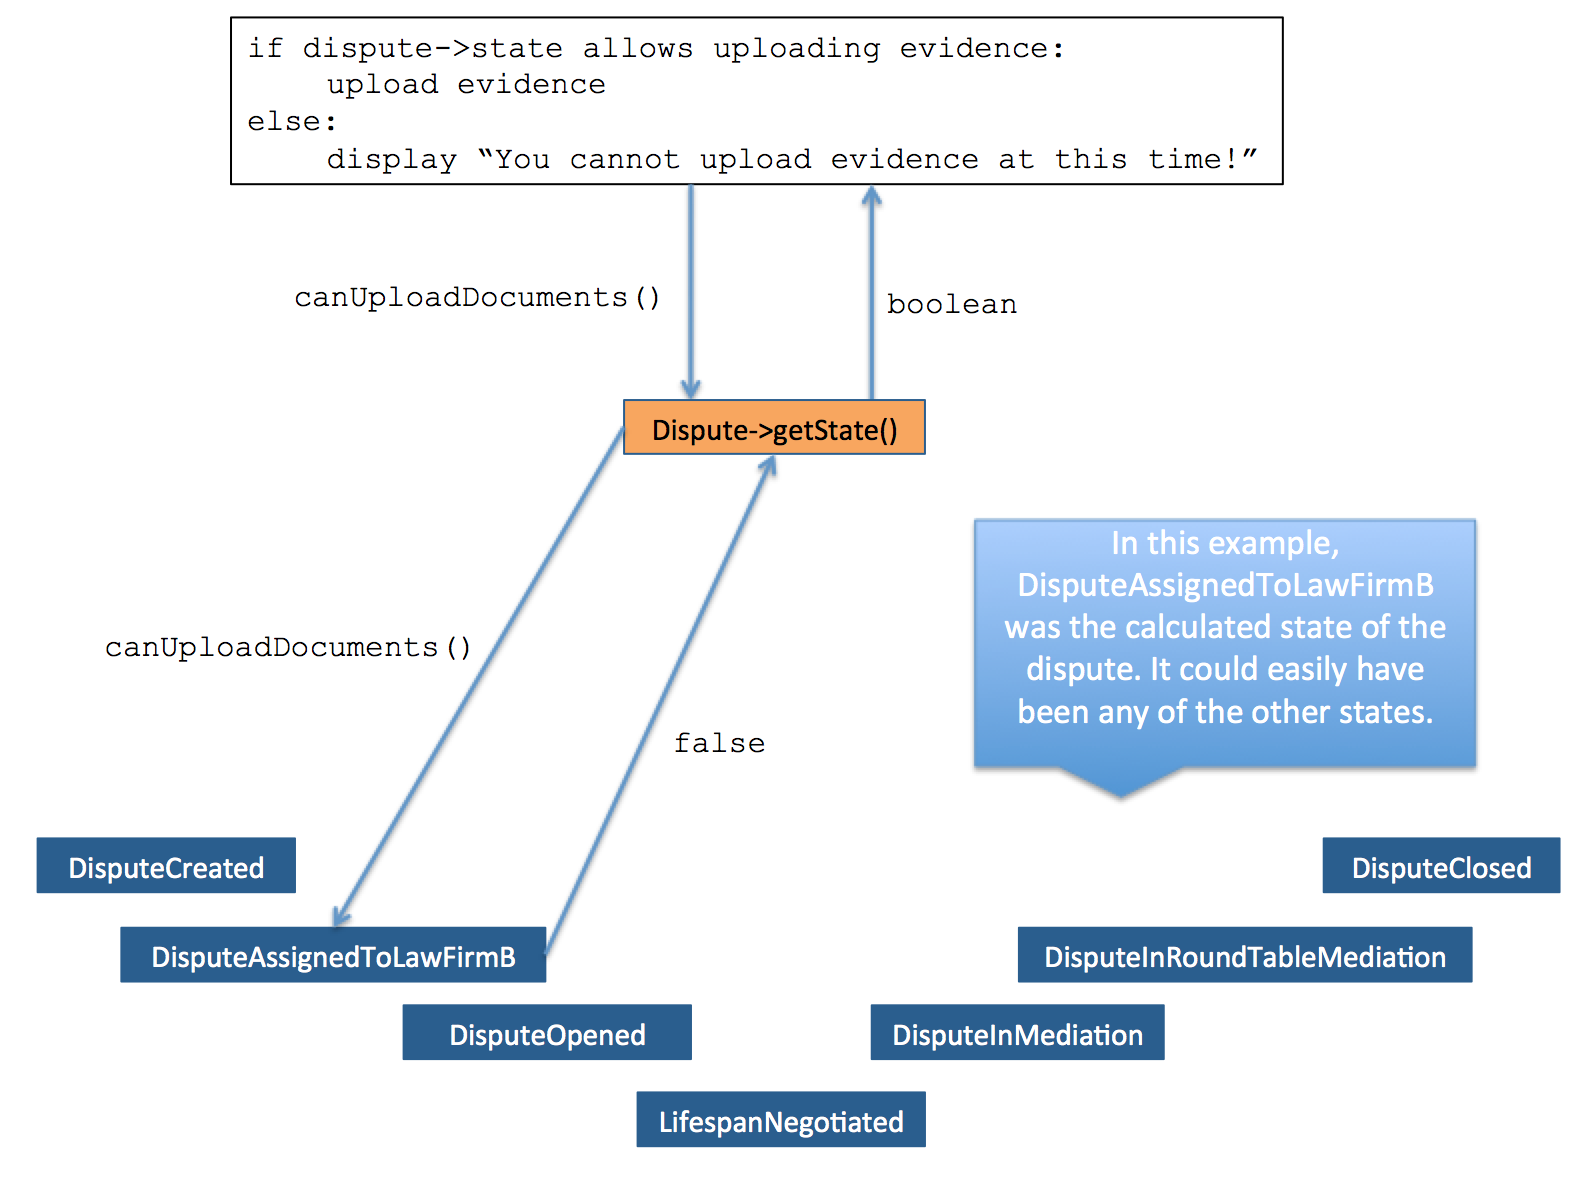
\includegraphics[width=\textwidth]{states}
    \fi
  \caption{Visualisation of how the state pattern works in SmartResolution}
  \label{uml:states}
\end{figure}

The list of possible states are as follows:

\begin{itemize}
    \item \textbf{DisputeCreated} - this is the very first state of the dispute, having just been created.
    \item \textbf{DisputeAssignedToLawFirmB} - this rather long-winded name represents the state of the dispute when it has just been assigned to the other law firm. At this stage, one dispute party is complete, whilst the other only has the law firm. We are still waiting for the law firm to assign an agent.
    \item \textbf{DisputeOpened} - all law firms and agents have been assigned. Now a lifespan must be negotiated.
    \item \textbf{LifespanNegotiated} - the agents have managed to negotiate a lifespan and there is nothing more to do to initiate the dispute. When the start date is surpassed, the dispute is underway and the agents are free to perform all dispute-related actions. When the end date passes, the dispute is automatically closed.
    \item \textbf{DisputeInMediation} - the agents have decided to put the dispute into mediation and have negotiated a mediation centre and a mediator. It is important to note that not all disputes will necessarily reach this stage.
    \item \textbf{DisputeInRoundTableMediation} - all parties are free to communicate openly. By default, a dispute in mediation disables direct communication between the two agents. The mediator can enable round-table communication to put the dispute into this state.
    \item \textbf{DisputeClosed} - the dispute is now closed, either because an agent closed it or because the lifespan of the dispute came to an end.
\end{itemize}


Also

@TODO - a class diagram showing all classes

Also

@TODO - describe in detail the models, data mappers and controller objects.

\section{Routing}

@TODO - before this point, describe the classes etc, since these are alluded to in the diagram.

\begin{figure}[h!]
  \centering
    \ifimages
    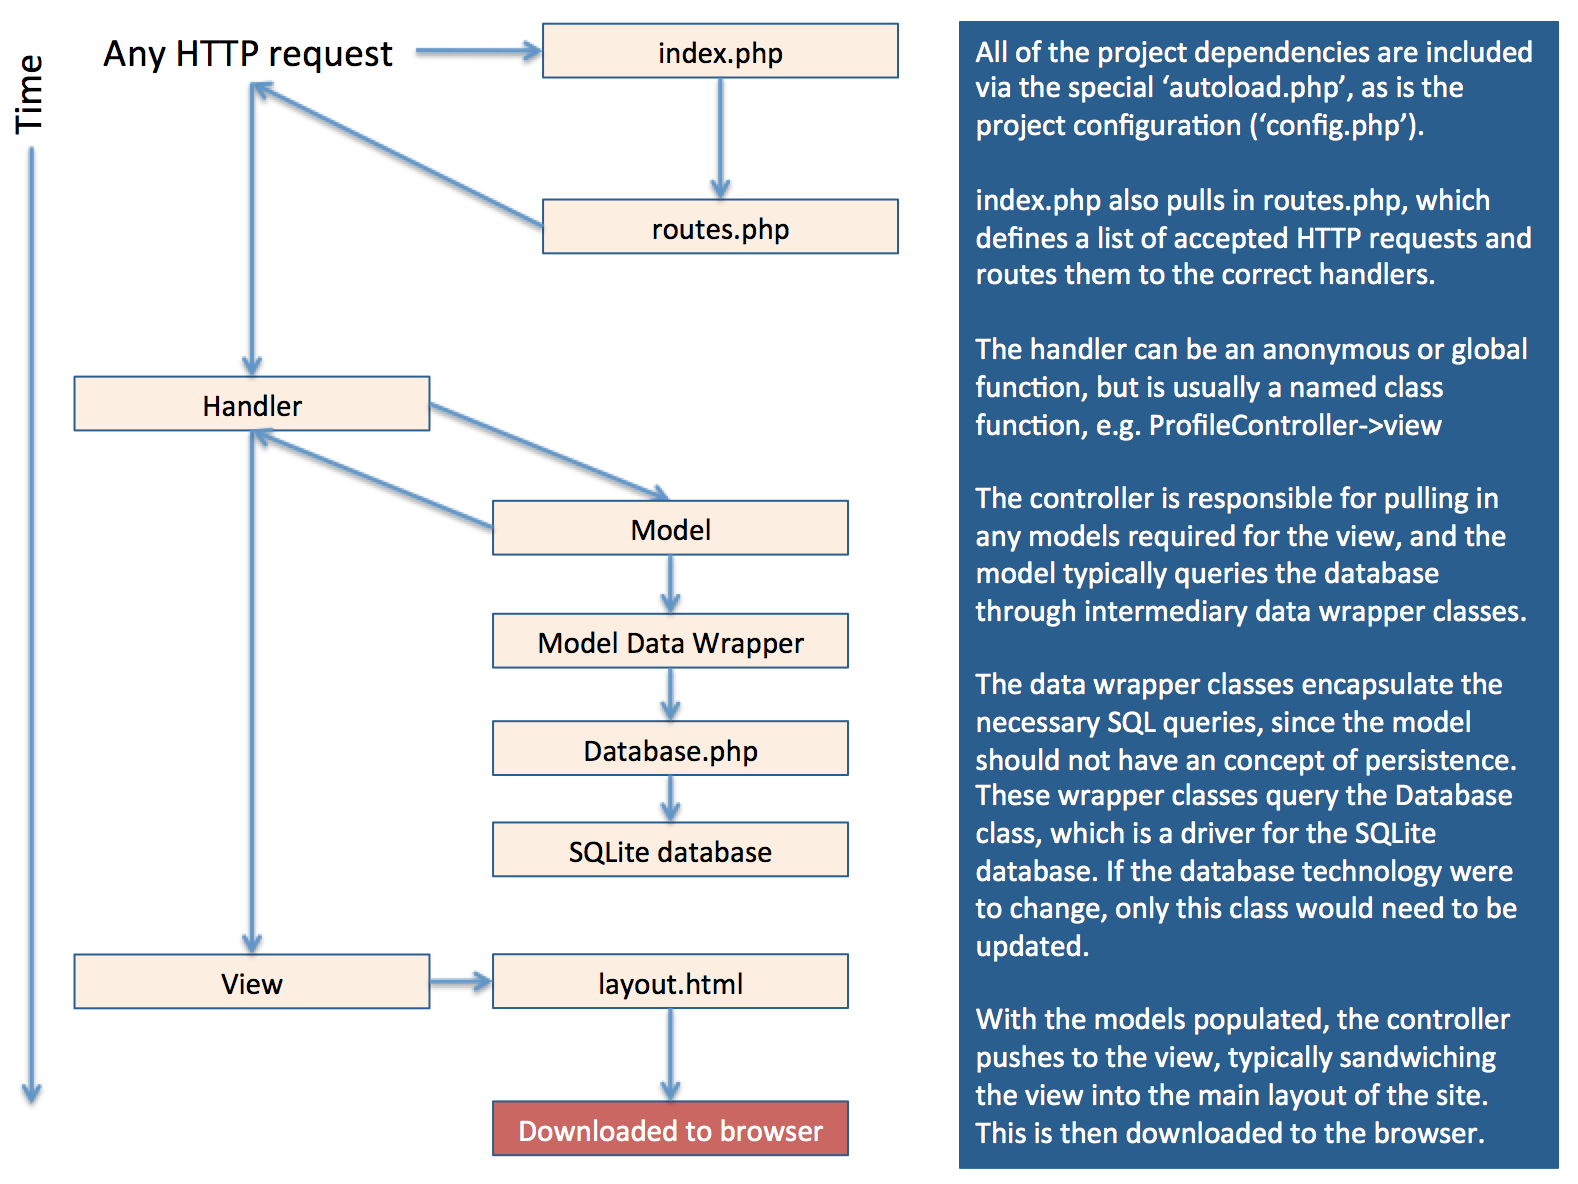
\includegraphics[width=\textwidth]{routing}
    \fi
  \caption{How SmartResolution processes HTTP requests}
  \label{uml:routing}
\end{figure}

Figure~\ref{uml:routing} shows how SmartResolution routes HTTP requests and renders data-driven pages. As described in the image, the HTTP request is processed by \lstinline{routes.php} and forwarded to the appropriate controller, which then instantiates the models and renders the view.

\section{Comments}

@TODO mention this somewhere:

The codebase is liberally commented throughout, using API-style markup. This was a difficult decision, discussed and justified in appendix~\ref{appendix:comments}.

\section{SmartResolution Marketplace}

@TODO mention somewhere that this was in a private repo, and why.

The SmartResolution website was developed locally using many of the same technologies as the core SmartResolution software, including F3, Bootstrap, Composer and so on. For the SmartResolution Marketplace functionality to be implemented, it was clear that the website would need to be deployed somewhere remotely.

\subsection{Choosing a server}

A local, physical server would not be practical for hosting the SmartResolution marketplace. If ever the platform became popular, it would not be able to cope with the numbers of people downloading the software (which weighs in at over 400KB) and browsing the documentation. Moreover, it is an unnecessary maintenance and upfront expense when so many alternatives exist.

Cloud computing as a web hosting service is becoming increasingly popular [REF], Amazon Web Services (AWS) chief amongst these in terms of exponential growth, being utilised by companies big and small, including the BBC. [REF] Its popularity is down to its speed and scalability, as well as the low cost to market.

AWS has server farms in X, Y and Z, supporting optimised regional sites, content delivery networks (CDNs) and so on. It can be configured to automatically deploy additional EC2 (Amazon Elastic Compute Cloud) instances when there is a surge in website traffic. This keeps the website online and responsive no matter how many HTTP requests are coming through.

Other alternatives exist, of course, such as Unlimited Web Hosting [REF], which is a cloud web hosting service I like to use for all of my personal projects. However, SmartResolution requires shell access for the installation process, in order to download dependencies through Composer, set up the SQLite database and so on.

AWS provides root access, and though other services also provide this facility (DigitalOcean, for example [REF]), it made sense to invest time in configuring an infrastructure that would be able to be expanded should the traffic require it in future.

\subsection{Configuring the server}

At the point where an EC2 instance is started, a dynamic IP address is generated, making the instance available at that given IP. By default, that IP address is not persistent and every 24 hours or so the IP addresses are reallocated and the instance must be reached through a different IP.

AWS offers an 'Elastic IP' facility, which allows you to generate a permanent IP address and allocate it to an EC2 instance. This costs a little extra but is a necessary step to ensure the website is always locatable.

Finally, Amazon's Route 53 service is a scalable DNS and allows you to link a domain name to an IP address, so that browsers querying that domain name are redirected to the content at the IP address endpoint, provided the domain name request is routed to Amazon's DNS.

smartresolution.org was purchased through the domain registrar gandi.net [REF] and the nameservers for Amazon's Route 53 service were specified as the DNS.

On the server itself, the EC2 instance is automatically deployed as a LAMP server running Amazon's own Linux [REF], Apache, MySQL and PHP.
%http://aws.amazon.com/amazon-linux-ami/

Early versions of the website were tightly coupled to the SmartResolution software itself as we ran a live demo on the site. This made it difficult to update the software on the website when the software was updated. The decision was made to separate the two concepts further, so that the demo would be available on a subdomain rather than the main site index.

To accomplish this, a VirtualHost was specified in the Apache configuration to redirect any requests for demo.smartresolution.org to a specific demo folder containing the SmartResolution software, which could then be easily updated as and when SmartResolution was updated.

All of this is demonstrated in figure~\ref{uml:serverConfig}.

\begin{figure}[h!]
  \centering
    \ifimages
    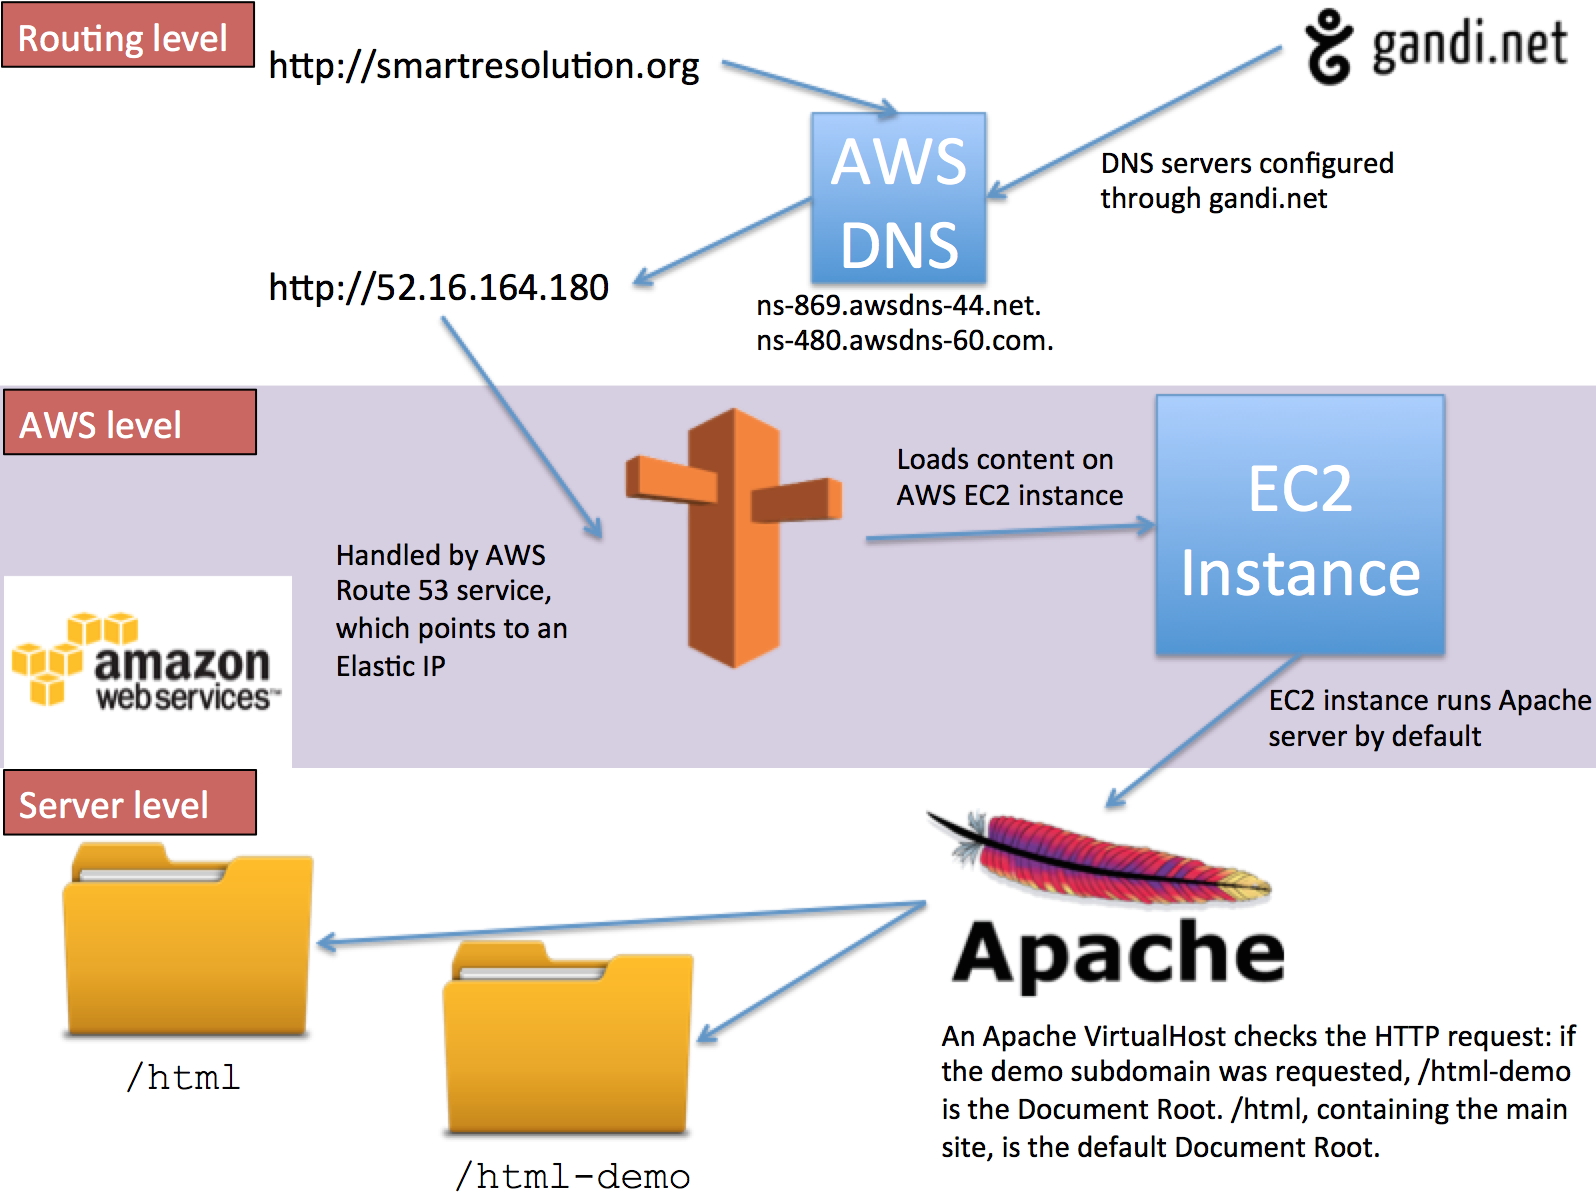
\includegraphics[width=\textwidth]{server_config}
    \fi
  \caption{The server configuration for smartresolution.org}
  \label{uml:serverConfig}
\end{figure}

\subsection{Continuous deployment}

Though continuous integration is important for ensuring that the codebase remains fully functional, continuous deployment is important for ensuring that the version of SmartResolution available for demo and for download on the SmartResolution website is fully up to date. It needed to be simple to keep both elements at the latest version.

I wrote a bash script specific to the SmartResolution vendor site which clears the html and html-demo folders outlined in figure~\ref{uml:serverConfig}, then re-downloads and installs the website and the software from the website repository and the software repository respectively.

In an ideal world, this script would be triggered via a Git web hook [REF] so that the website is updated whenever an update is pushed to either the website or software repository. However, triggering this bash script through PHP is a security issue and is by default made very difficult to accomplish through AWS' default Apache and PHP configuration. After some failed attempts and with time pressing on, it was decided that manually signing into the EC2 instance and running the update script was not too much of an inconvenience.

The script can be found at appendix X @TODO?? (this will be part of the technical hand-in so perhaps isn't needed here)